%\subsection{Effect of lens radium}
%lensed_waveguide_radium
In this part the effect of the radium of the lens interface for the waveguide will be discussed. We are going to keep the height of the lens on the waveguide and change the lens radium. In Tab. \ref{tab:coupling_lensed_waveguide_radium} the lens height is chosen for $1\mu$m, $1.5\mu$m and $2\mu$m respectively. We expand the lens radium from $2\mu$m to $3.6\mu$m and observe $|S21|$ as coupling efficiency.\\

\begin{table}
\caption{Cupling efficiency between TLF and lensed waveguide due to changing the lens radium}
\centering
\begin{tabular}{|c|c|c|c|}
\hline
\multirow{2}*{Radium($\mu$m)}&\multicolumn{3}{c|}{Height($\mu$m)}\\
\cline{2-4}
 								&	1&	1.5&2\\
\hline
$2.0$& $59.5\%$	&$61.3\%$	&$69\%$\\
$2.2$& $59\%$		&$60.8\%$	&$68.3\%$\\
$2.4$&$59\%$		&$60.3\%$	&$66.8\%$\\
$2.6$&$58.6\%$	&$59.9\%$	&$65.3\%$\\
$2.8$&$58.2\%$	&$59.3\%$	&$64\%$\\
$3.0$&$57.8\%$	&$58.7\%$	&$63\%$\\
\hline
\end{tabular}
\label{tab:coupling_lensed_waveguide_radium}
\end{table}

According the data in Tab. \ref{tab:coupling_lensed_waveguide_radium} the coupling behavior curve can be mapped in Fig. \ref{fig:coupling_lenses_curve_rxx}. Apparently, it can be told that the coupling efficiencies under different lens heights are monotonously declining due to the variation of the lens radium.
\begin{figure}[!ht]
\centering
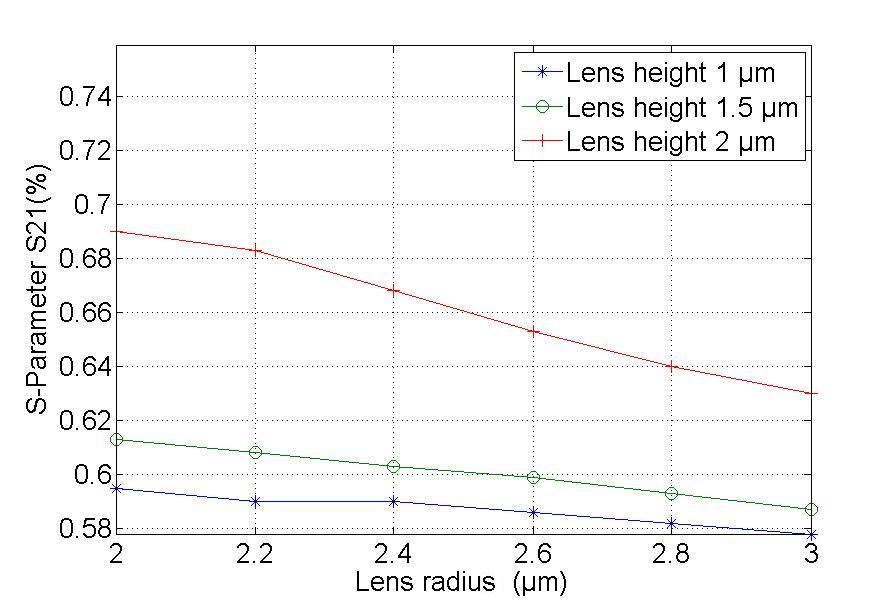
\includegraphics[width=0.8\textwidth]{bilder/s21_fix_lens_height_rxx}
\caption{Coupling efficiency due to changing the lens radium}
\label{fig:coupling_lenses_curve_rxx}
\end{figure}
\begin{figure}[!ht]
\centering
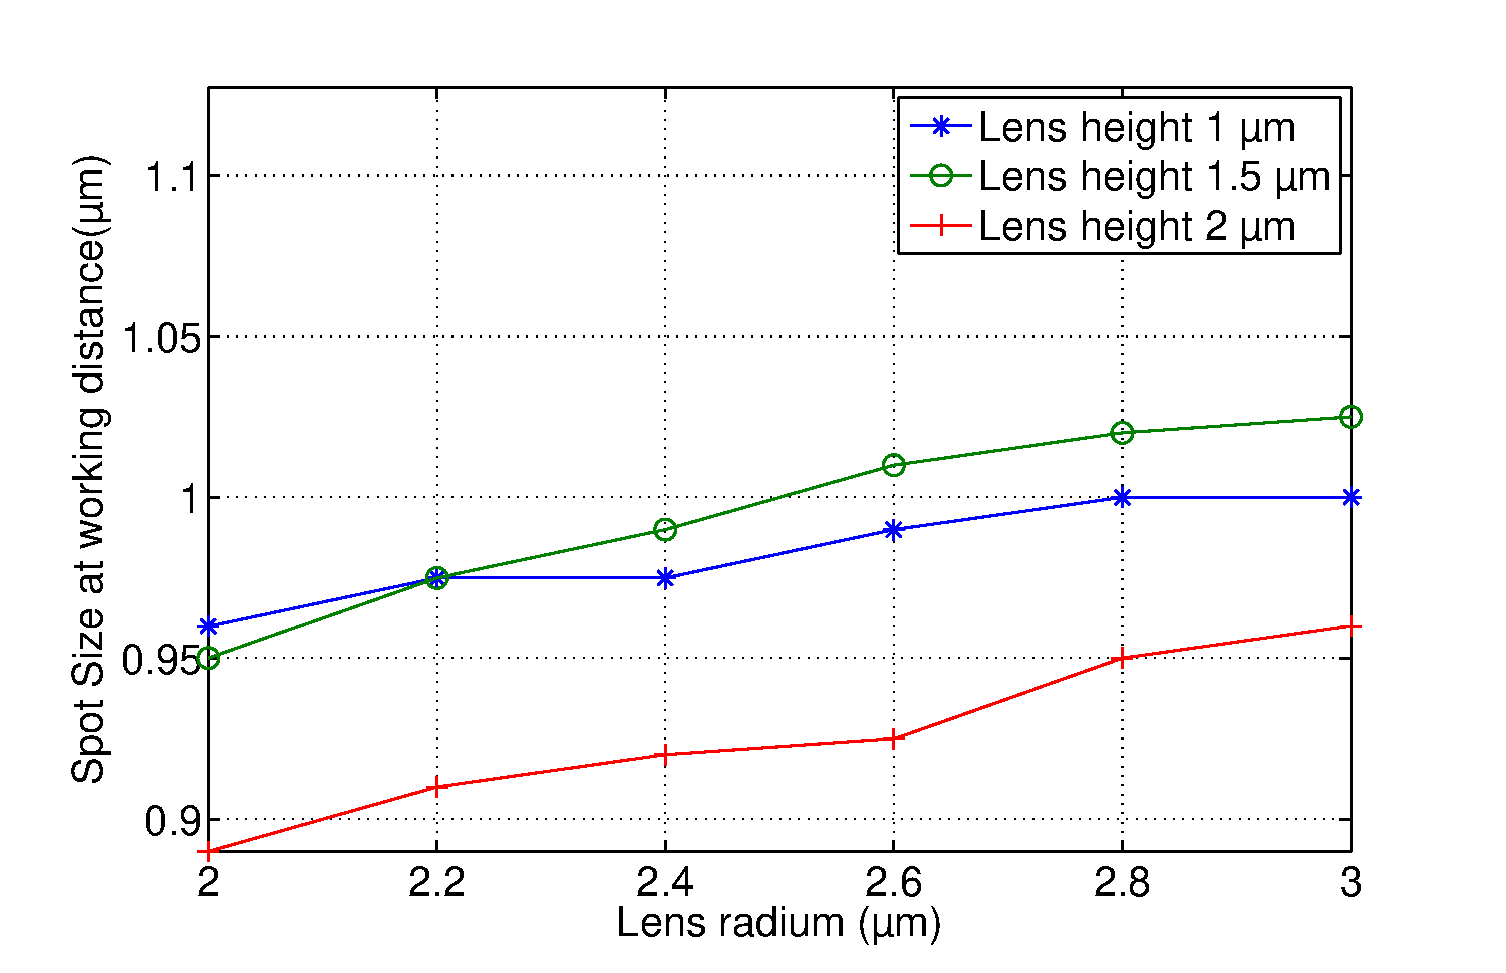
\includegraphics[width=0.8\textwidth]{bilder/spot_fix_lens_height_rxx}
\caption{The spot size curve at lensed waveguide interface due to changing lens height}
\label{fig:lensed_guide_spot_size_curve_rxx}
\end{figure}
At the mean time the spot size curve in Fig. \ref{fig:lensed_guide_spot_size_curve_rxx} along the variation of the lens radium behave inversely in compare with the trends of coupling efficiency. These simulation results bring us the conclusion that the smallest lens radium gains the best coupling efficiency when the lens height is fixed. 
